\documentclass[11pt]{article}

\usepackage[margin=0.9in]{geometry}
\usepackage[T1]{fontenc}
\usepackage{lmodern}
\usepackage{microtype}
\usepackage{parskip}
\usepackage{booktabs}
\usepackage{tabularx}
\usepackage{array}
\usepackage{enumitem}
\usepackage{needspace}
\usepackage{xcolor}
\usepackage{listings}
\usepackage{tikz}
\usetikzlibrary{arrows.meta,positioning,fit,calc}
\usepackage[most]{tcolorbox}
\usepackage{fancyhdr}
\usepackage{hyperref}

\definecolor{PhorosNavy}{HTML}{16324F}
\definecolor{PhorosBlue}{HTML}{246B8E}
\definecolor{PhorosTeal}{HTML}{1E7A72}
\definecolor{PhorosGold}{HTML}{C28A2C}
\definecolor{PhorosLight}{HTML}{F2F6F8}
\definecolor{PhorosLine}{HTML}{C9D7DE}
\definecolor{CodeBg}{HTML}{F7F9FA}
\definecolor{CodeComment}{HTML}{5E746D}

\hypersetup{
  colorlinks=true,
  linkcolor=PhorosBlue,
  urlcolor=PhorosBlue,
  pdftitle={Source Artifact Model},
  pdfauthor={Phoros}
}

\pagestyle{fancy}
\fancyhf{}
\fancyhead[L]{\small\color{PhorosNavy}Source Artifact Model}
\fancyhead[R]{\small\color{PhorosBlue}Phoros Architecture}
\fancyfoot[C]{\small\thepage}
\renewcommand{\headrulewidth}{0.3pt}
\setlength{\headheight}{14pt}

\setlist[itemize]{leftmargin=1.4em,itemsep=0.25em,topsep=0.4em}
\setlist[enumerate]{leftmargin=1.6em,itemsep=0.35em,topsep=0.4em}

\lstdefinelanguage{Rust}{
  morekeywords={pub,struct,enum,trait,impl,fn,type,where,match,Self,self,Option,Some,None,Vec,String,u8,u32,u64,bool},
  sensitive=true,
  morecomment=[l]{//},
  morecomment=[s]{/*}{*/},
  morestring=[b]"
}

\lstset{
  language=Rust,
  basicstyle=\ttfamily\footnotesize,
  keywordstyle=\color{PhorosBlue}\bfseries,
  commentstyle=\color{CodeComment}\itshape,
  stringstyle=\color{PhorosTeal},
  backgroundcolor=\color{CodeBg},
  frame=single,
  rulecolor=\color{PhorosLine},
  framerule=0.5pt,
  xleftmargin=0.5em,
  framexleftmargin=0.5em,
  xrightmargin=0.5em,
  framexrightmargin=0.5em,
  breaklines=true,
  columns=fullflexible,
  keepspaces=true,
  showstringspaces=false,
  aboveskip=0.8em,
  belowskip=0.8em
}

\newtcolorbox{principlebox}[1][]{
  colback=PhorosLight,
  colframe=PhorosBlue,
  boxrule=0.7pt,
  arc=2pt,
  left=8pt,right=8pt,top=7pt,bottom=7pt,
  fonttitle=\bfseries,
  title=#1
}

\newtcolorbox{decisionbox}[1][]{
  colback=white,
  colframe=PhorosTeal,
  boxrule=0.7pt,
  arc=2pt,
  left=8pt,right=8pt,top=7pt,bottom=7pt,
  fonttitle=\bfseries,
  title=#1
}

\newcommand{\code}[1]{\texttt{#1}}
\newcommand{\term}[1]{\textbf{#1}}

\title{\vspace{-2.5em}\color{PhorosNavy}\textbf{Source Artifact Model}\\[0.35em]
\large Preserving Immutable Healthcare Evidence Before FEN Interpretation}
\author{Phoros Architecture Note}
\date{August 21, 2026}

\begin{document}

\maketitle

\begin{principlebox}[The idea in one sentence]
A \code{SourceArtifact} does not contain document bytes. It is an immutable Rust domain record that reaches those bytes through a typed \code{StoredObjectRef}; processing runs interpret the preserved bytes, and FEN facts record the resulting semantic assertions.
\end{principlebox}

\setcounter{tocdepth}{1}
\begingroup
\footnotesize
\setlength{\parskip}{0pt}
\tableofcontents
\endgroup
\newpage

\section{Begin With One PDF}

Suppose Phoros receives a file named \code{medical-record.pdf}. Before considering parsers, FEN facts, or compound archives, ask the simplest question: \emph{where do the PDF bytes live?}

The answer is: in protected object storage. Neither \code{SourceArtifact} nor \code{StoredObjectRef} contains the PDF bytes inside the Rust value.

\begin{center}
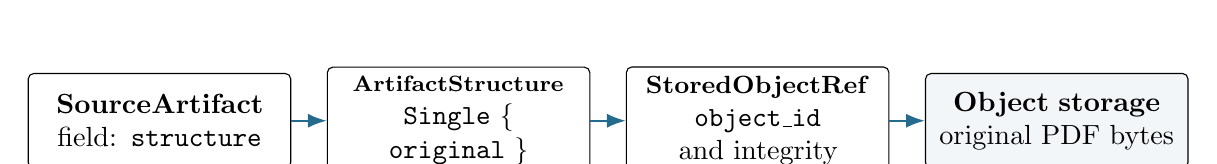
\begin{tikzpicture}[
  node distance=0.45cm,
  box/.style={draw, rounded corners=2pt, text width=3.1cm, minimum height=1.2cm, align=center, fill=white},
  bytes/.style={draw, rounded corners=2pt, text width=3.1cm, minimum height=1.2cm, align=center, fill=PhorosLight},
  arrow/.style={-{Latex[length=2.4mm]}, thick, color=PhorosBlue}
]
  \node[box] (artifact) {\textbf{SourceArtifact}\\field: \code{structure}};
  \node[box, right=of artifact] (structure) {\textbf{\footnotesize ArtifactStructure}\\\code{Single \{ original \}}};
  \node[box, right=of structure] (reference) {\textbf{\small StoredObjectRef}\\\code{object\_id} and integrity};
  \node[bytes, right=of reference] (bytes) {\textbf{Object storage}\\original PDF bytes};

  \draw[arrow] (artifact) -- (structure);
  \draw[arrow] (structure) -- (reference);
  \draw[arrow] (reference) -- (bytes);
\end{tikzpicture}
\end{center}

Read the diagram from left to right:

\begin{enumerate}
  \item \code{SourceArtifact} records the receipt event: account, time, provenance, authority, supplied metadata, and structure.
  \item Its \code{structure} field is \code{ArtifactStructure::Single} because the received source is one PDF.
  \item The variant's \code{original} field is a \code{StoredObjectRef}. This small Rust value identifies the stored object and carries its digest, length, media type, and protection reference.
  \item A storage adapter uses that reference to retrieve and decrypt the actual PDF bytes from object storage.
\end{enumerate}

\begin{decisionbox}[The most important boundary]
The \code{SourceArtifact} contains an \code{ArtifactStructure}; the structure contains a \code{StoredObjectRef}; object storage contains the PDF bytes. The word ``contains'' means something different at each step.
\end{decisionbox}

\subsection{The nesting in Rust}

The relevant types, stripped of unrelated fields, are:

\begin{lstlisting}
pub struct StoredObjectRef {
    pub object_id: StoredObjectId,
    pub digest: ContentDigest,
    pub byte_length: u64,
    pub media_type: MediaType,
    pub protection: ProtectionRef,
}

pub enum ArtifactStructure {
    Single {
        original: StoredObjectRef,
    },
    // Compound is introduced later.
}

pub struct SourceArtifact {
    // receipt context omitted here
    pub structure: ArtifactStructure,
}
\end{lstlisting}

Conceptually, a received PDF therefore has this shape:

\begin{lstlisting}
SourceArtifact {
    structure: ArtifactStructure::Single {
        original: StoredObjectRef {
            object_id: /* lookup key for protected storage */,
            digest: /* hash of the exact PDF bytes */,
            byte_length: /* size of the PDF */,
            media_type: /* application/pdf */,
            protection: /* how access is authorized */,
        },
    },
    // receipt context omitted here
}
\end{lstlisting}

The retrieval path is thus:

\begin{lstlisting}
artifact.structure
    -> Single.original
    -> StoredObjectRef.object_id
    -> object-store lookup and authorized decryption
    -> original PDF bytes
\end{lstlisting}

\subsection{Four similar terms with different meanings}

\begin{center}
\begin{tabularx}{\textwidth}{>{\bfseries}p{0.23\textwidth} X}
\toprule
Term & What it is \\
\midrule
\code{SourceArtifact} & The immutable domain record for one received source event. It has provenance and a nested reference to the original bytes. \\
\code{ArtifactStructure} & The typed description of whether the source is one object or a compound container. \\
\code{StoredObjectRef} & A small Rust value that identifies protected bytes and records how to verify them. It is not the byte payload. \\
Stored object & The protected byte object held by the storage system; for this example, it is the exact PDF that arrived. \\
\bottomrule
\end{tabularx}
\end{center}

\section{Why Separate the Record From the Bytes?}

Healthcare information reaches a patient in forms designed by many different institutions: PDFs, portal downloads, email attachments, claims files, FHIR bundles, and large electronic health information (EHI) exports. Phoros needs to preserve these sources before it attempts to understand them.

The separation lets the domain model remain small and testable while a storage adapter handles streaming, encryption, authorization, and provider-specific object locations. It also prevents large or sensitive payloads from being copied through ordinary domain operations.

That ordering matters. A parser can be improved. A coding rule can change. An extraction model can be replaced. The bytes that actually arrived must remain stable so that every later interpretation can be reproduced, challenged, or corrected.

The source artifact model therefore has three responsibilities:

\begin{enumerate}
  \item preserve exactly what was received;
  \item record how, when, and under what authority it was received; and
  \item provide precise citations for processing results and FEN facts.
\end{enumerate}

It deliberately does \emph{not} decide what the source means clinically or economically. Meaning belongs to processing and FEN.

\section{From Preserved Bytes to FEN Facts}

After the PDF boundary is clear, the larger model has three stages: preserved evidence, repeatable interpretation, and semantic state.

\begin{center}
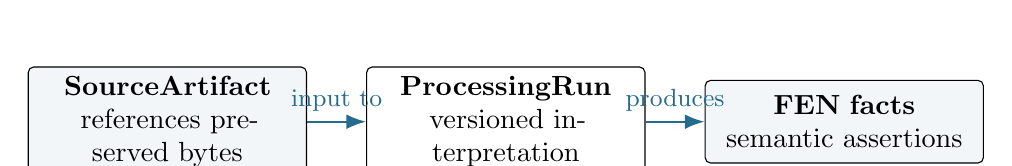
\begin{tikzpicture}[
  node distance=0.75cm,
  box/.style={draw, rounded corners=2pt, text width=3.3cm, minimum height=1.05cm, align=center, fill=white},
  arrow/.style={-{Latex[length=2.5mm]}, thick, color=PhorosBlue}
]
  \node[box, fill=PhorosLight] (artifact) {\textbf{SourceArtifact}\\references preserved bytes};
  \node[box, right=of artifact] (run) {\textbf{ProcessingRun}\\versioned interpretation};
  \node[box, right=of run, fill=PhorosLight] (fact) {\textbf{FEN facts}\\semantic assertions};

  \draw[arrow] (artifact) -- node[above, font=\small]{input to} (run);
  \draw[arrow] (run) -- node[above, font=\small]{produces} (fact);
\end{tikzpicture}
\end{center}

A \code{SourceCitation} connects a produced fact back through its processing run to the precise artifact, and optionally to a page, archive member, row, or field.

\begin{center}
\begin{tabularx}{\textwidth}{>{\bfseries}p{0.23\textwidth} X}
\toprule
Object & Question it answers \\
\midrule
\code{SourceArtifact} & What evidence did Phoros receive, for which account, and with what provenance? \\
\code{StoredObjectRef} & Which protected byte object holds the source, and how can those bytes be verified? \\
\code{ProcessingRun} & Which parser or model interpreted the evidence, using which version and configuration? \\
\code{SourceCitation} & What exact part of the evidence supports this output? \\
FEN fact & What semantic assertion did Phoros accept into the patient record? \\
\bottomrule
\end{tabularx}
\end{center}

\section{Identity Is Not a Content Hash}

A content hash is excellent for integrity, but it is the wrong identity for a source artifact.

Suppose the same PDF arrives once from a provider portal and later as an email attachment. The bytes may be identical, but Phoros observed two distinct deliveries with different timestamps, channels, and authorization histories. Those deliveries should produce two \code{SourceArtifactId} values even if storage deduplicates their bytes.

\begin{lstlisting}
pub struct SourceArtifactId(pub String);
pub struct StoredObjectId(pub String);

pub struct ContentDigest {
    pub algorithm: DigestAlgorithm,
    pub value: Vec<u8>,
}

pub enum DigestAlgorithm {
    Sha256,
}
\end{lstlisting}

\begin{principlebox}[Identity rule]
\code{SourceArtifactId} identifies an evidentiary occurrence. \code{ContentDigest} identifies byte content. Storage may deduplicate content without collapsing receipt history.
\end{principlebox}

\section{The Stored-Byte Boundary}

The domain model should not expose filesystem paths, cloud URLs, credentials, raw encryption keys, or an in-memory byte vector. It retains only a provider-neutral reference and the information needed to verify the retrieved bytes.

\begin{lstlisting}
pub struct StoredObjectRef {
    pub object_id: StoredObjectId,
    pub digest: ContentDigest,
    pub byte_length: u64,
    pub media_type: MediaType,
    pub protection: ProtectionRef,
}

pub struct MediaType {
    pub value: String,
}

pub struct ProtectionRef(pub String);
\end{lstlisting}

The \code{object\_id} is resolved by a storage adapter; it is not necessarily a path or URL. The digest is computed over the exact original plaintext bytes before encryption. Encryption metadata and key resolution belong to the storage adapter.

The digest itself should still be treated as sensitive operational metadata because a known-file attack can reveal that an account holds a particular document.

\section{The Immutable Core}

The central aggregate is intentionally small. It records stable receipt context and a nested route to the evidence; it does not embed the evidence payload or conclusions produced later.

\begin{lstlisting}
pub struct SourceArtifact {
    pub id: SourceArtifactId,
    pub account_id: AccountId,
    pub received_at: Timestamp,
    pub receipt: ReceiptProvenance,
    pub authorization: AcquisitionAuthority,
    pub structure: ArtifactStructure,
    pub supplied_metadata: SuppliedMetadata,
}
\end{lstlisting}

There is deliberately no \code{pdf: Vec<u8>} or \code{bytes: Vec<u8>} field. For the PDF example, the route to the bytes begins at \code{structure}, continues through \code{ArtifactStructure::Single.original}, and ends at the referenced stored object.

\subsection{Why the account is required but the subject is not}

The receiving endpoint belongs to a Phoros account, so account ownership is known at receipt time. The people or other semantic subjects mentioned in a document may not yet be known. Determining them is an interpretation step.

Requiring \code{SubjectId} during receipt would encourage the ingestion layer to guess. Subject associations should instead be recorded later with their evidence and confidence.

\subsection{What immutability means}

Once finalized, the aggregate is never edited in place. In particular, the following remain stable:

\begin{itemize}
  \item the original object reference and digest;
  \item the trusted receipt timestamp and receiving endpoint;
  \item the metadata supplied with the delivery; and
  \item the acquisition authority recorded at receipt.
\end{itemize}

Later knowledge is appended as a separate observation. For example, a sender may be claimed at receipt and verified later. The verification does not rewrite the original claim.

\Needspace{0.55\textheight}
\section{Extending the PDF Model: Single and Compound}

The PDF example establishes the single case. A ZIP export changes only the \code{ArtifactStructure} variant; the surrounding \code{SourceArtifact} still records one receipt event.

\begin{lstlisting}
pub enum ArtifactStructure {
    Single {
        original: StoredObjectRef,
    },
    Compound {
        original: StoredObjectRef,
        manifest: ArtifactManifest,
    },
}
\end{lstlisting}

For a PDF, \code{Single.original} is the \code{StoredObjectRef} for the exact PDF bytes. For an Epic EHI ZIP, \code{Compound.original} is the \code{StoredObjectRef} for the exact ZIP bytes, while \code{manifest} describes a verified decomposition of the archive.

\begin{decisionbox}[What stays authoritative]
The original reference always resolves to exactly what arrived: PDF bytes in the single case and ZIP bytes in the compound case. A manifest and any extracted member objects improve inspection and processing; they do not replace the original archive as evidence.
\end{decisionbox}

\begin{lstlisting}
pub struct ArtifactManifest {
    pub format: ContainerFormat,
    pub members: Vec<ArtifactMember>,
}
\end{lstlisting}

\Needspace{0.18\textheight}
\begin{lstlisting}
pub enum ContainerFormat {
    Zip,
    Tar,
    GzipTar,
    Other(String),
}
\end{lstlisting}

\Needspace{0.28\textheight}
\begin{lstlisting}
pub struct ArtifactMember {
    pub id: ArtifactMemberId,
    pub relative_path: String,
    pub uncompressed_length: u64,
    pub digest: ContentDigest,
    pub detected_media_type: Option<MediaType>,
    pub extracted_object: Option<StoredObjectRef>,
}
\end{lstlisting}

The member digest proves the extracted bytes. The optional extracted-object reference allows efficient processing without making the extracted copy a new source event. The archive remains authoritative.

\subsection{Why a manifest is useful}

For a large EHI export, the manifest enables Phoros to:

\begin{itemize}
  \item verify that extraction produced the expected members;
  \item process one table without repeatedly expanding the archive;
  \item detect missing, duplicate, or changed members;
  \item cite a stable member identity instead of relying on a filename alone; and
  \item preserve directory relationships and documentation shipped with the export.
\end{itemize}

Archive inspection must be bounded. Member counts, expanded byte totals, path traversal, nested archives, and compression ratios require defensive limits before an artifact is finalized as compound.

\section{Receipt Provenance and Authority}

Provenance must distinguish what the sender claimed from what Phoros verified.

\begin{lstlisting}
pub struct ReceiptProvenance {
    pub channel: ReceiptChannel,
    pub endpoint_id: CommunicationsEndpointId,
    pub external_message_id: Option<String>,
    pub claimed_sender: Option<String>,
    pub transport_evidence: Vec<TransportEvidenceRef>,
}
\end{lstlisting}

\Needspace{0.20\textheight}
\begin{lstlisting}
pub enum ReceiptChannel {
    SecureUpload,
    Smtp,
    DirectMessaging,
    Fhir,
    ProviderApi,
    LocalImport,
}
\end{lstlisting}

\Needspace{0.22\textheight}
\begin{lstlisting}
pub enum AcquisitionAuthority {
    PatientProvided,
    PatientDirectedDisclosure,
    HipaaRightOfAccess,
    AuthorizedAccountManager,
    Other(AuthorityEvidenceRef),
}
\end{lstlisting}

The exact authority taxonomy may evolve. The important initial rule is that acquisition authority is typed and evidence-bearing rather than an unstructured note.

\begin{decisionbox}[Claim versus verification]
An email header may claim a sender. A Direct signature or provider API credential may verify one. Store the claim in the immutable receipt record and append verification results separately; never silently promote a claim into a verified identity.
\end{decisionbox}

\Needspace{0.55\textheight}
\section{Processing Is Separate and Repeatable}

A processing run records one attempt to interpret an artifact. It is not part of the immutable artifact because the same source can be processed repeatedly as software improves.

\begin{lstlisting}
pub struct ProcessingRun {
    pub id: ProcessingRunId,
    pub artifact_id: SourceArtifactId,
    pub processor: ProcessorIdentity,
    pub configuration_ref: Option<String>,
    pub started_at: Timestamp,
    pub completed_at: Option<Timestamp>,
    pub outcome: ProcessingOutcome,
}

pub struct ProcessorIdentity {
    pub name: String,
    pub version: String,
}

pub enum ProcessingOutcome {
    Running,
    Succeeded,
    SucceededWithWarnings,
    Failed { error_code: String },
}
\end{lstlisting}

Processing should be reproducible from the artifact digest, processor version, and configuration. Nondeterministic systems, including AI models, should additionally record the model identity and any sampling or prompt-profile information needed to explain the result.

\Needspace{0.34\textheight}
\section{Citing Exact Evidence}

A source citation joins a processing result to the evidence that supports it.

\begin{lstlisting}
pub struct SourceCitation {
    pub artifact_id: SourceArtifactId,
    pub member_id: Option<ArtifactMemberId>,
    pub location: SourceLocation,
    pub processing_run_id: ProcessingRunId,
}
\end{lstlisting}

\Needspace{0.30\textheight}
\begin{lstlisting}
pub enum SourceLocation {
    WholeArtifact,
    PdfPage {
        page_number: u32,
    },
    DelimitedField {
        data_row: u64,
        column_name: String,
    },
    JsonPointer {
        pointer: String,
    },
    ByteRange {
        start: u64,
        length: u64,
    },
}
\end{lstlisting}

The citation is format-aware enough to be useful to a reviewer but does not embed parsed healthcare meaning. It says where evidence is located, not what that evidence means.

\section{Worked Example: Epic EHI Export}

Assume an account receives \code{patient-export.zip}. The archive contains \code{Claims.csv}, and row 842 has an \code{allowed\_amount} value of \code{12500} minor currency units.

\begin{center}
\begin{tikzpicture}[
  node distance=0.8cm,
  flowstep/.style={draw, rounded corners=2pt, text width=2.55cm, minimum height=1.0cm, align=center, fill=white},
  arrow/.style={-{Latex[length=2.2mm]}, thick, color=PhorosBlue}
]
  \node[flowstep, fill=PhorosLight] (zip) {EHI ZIP\\original archive};
  \node[flowstep, right=0.35cm of zip] (csv) {\code{Claims.csv}\\manifest member};
  \node[flowstep, right=0.35cm of csv] (cell) {row 842\\{\footnotesize\ttfamily allowed\_amount}};
  \node[flowstep, right=0.35cm of cell, fill=PhorosLight] (parser) {Epic parser\\version 1.4};
  \node[flowstep, right=0.35cm of parser] (fen) {FEN billing fact\\allowed = \$125.00};

  \draw[arrow] (zip) -- (csv);
  \draw[arrow] (csv) -- (cell);
  \draw[arrow] (cell) -- (parser);
  \draw[arrow] (parser) -- (fen);
\end{tikzpicture}
\end{center}

The resulting fact cites the artifact, the \code{Claims.csv} member, row 842, the named column, and processing run 1.4.

Later, parser version 1.5 discovers that the table's currency column must also be consulted. It creates a new processing run and may produce a corrected or superseding FEN fact. Nothing about the original ZIP, manifest, or row is rewritten.

\begin{principlebox}[The audit question]
For any derived FEN fact, Phoros should be able to answer: ``Which exact evidence did we read, and which versioned process turned it into this assertion?''
\end{principlebox}

\Needspace{0.25\textheight}
\section{Lifecycle Without Mutation}

Immutability applies to the evidence record, not to every operational decision around it.

\begin{center}
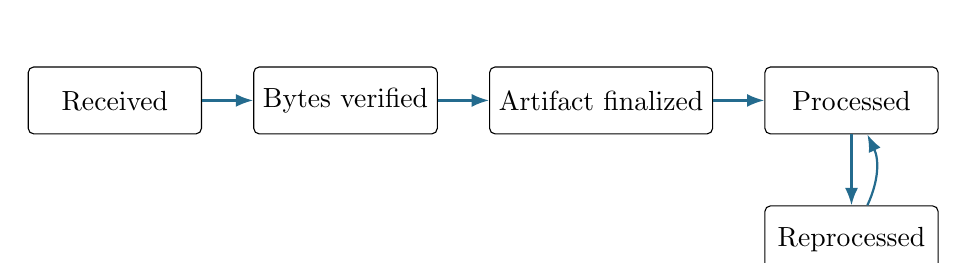
\begin{tikzpicture}[
  node distance=0.65cm,
  state/.style={draw, rounded corners=2pt, minimum width=2.2cm, minimum height=0.85cm, align=center},
  arrow/.style={-{Latex[length=2.2mm]}, thick, color=PhorosBlue}
]
  \node[state] (received) {Received};
  \node[state, right=of received] (verified) {Bytes verified};
  \node[state, right=of verified] (finalized) {Artifact finalized};
  \node[state, right=of finalized] (processed) {Processed};
  \node[state, below=0.9cm of processed] (reprocessed) {Reprocessed};

  \draw[arrow] (received) -- (verified);
  \draw[arrow] (verified) -- (finalized);
  \draw[arrow] (finalized) -- (processed);
  \draw[arrow] (processed) -- (reprocessed);
  \draw[arrow] (reprocessed) to[bend right=25] (processed);
\end{tikzpicture}
\end{center}

Receipt may use a short-lived staging record while bytes are uploaded, hashed, scanned, and---for archives---safely inspected. The immutable \code{SourceArtifact} is committed atomically only after its object references and manifest are complete.

Quarantine, access suspension, retention schedules, legal holds, and deletion are separate lifecycle records. They do not mutate the evidentiary claim about what arrived.

\subsection{Deletion and tombstones}

``Immutable'' should mean unchangeable while retained, not impossible to delete when law, policy, or patient direction requires deletion. A purge operation should remove the protected bytes and append a non-sensitive audit tombstone containing the artifact ID, deletion authority, time, and outcome. It must not imply that the bytes remain retrievable.

\section{Domain Invariants}

The first implementation should enforce the following rules at construction time:

\begin{enumerate}
  \item Every artifact has an opaque identity and a owning account.
  \item Every stored object has a tagged digest and byte length.
  \item A finalized artifact references only successfully persisted objects.
  \item A compound artifact retains the exact original container.
  \item Every manifest member has a safe relative path, stable member identity, digest, and length.
  \item Member identities are unique within a manifest.
  \item Extraction limits are checked before finalization.
  \item A processing run identifies one exact artifact and processor version.
  \item A citation's member belongs to the cited artifact.
  \item Storage deduplication never merges source-artifact receipt records.
\end{enumerate}

These invariants belong in constructors and repository boundaries rather than being left to application convention.

\Needspace{0.28\textheight}
\section{Security and Privacy Boundaries}

Source artifacts will often contain direct identifiers and dense protected health information. The source domain should therefore assume that content and much of its metadata are sensitive.

\begin{itemize}
  \item Encrypt original and extracted objects with account-scoped protection.
  \item Encrypt manifests when filenames or directory structure can reveal health information.
  \item Keep searchable operational metadata minimal.
  \item Require authorization before issuing a read capability or decryption operation.
  \item Audit access to originals independently from access to derived FEN facts.
  \item Treat malware scanning and archive inspection as untrusted-input boundaries.
  \item Never place storage credentials or public object URLs in domain values.
\end{itemize}

The domain can define a \code{SourceArtifactRepository} and an object-read authorization contract without depending on PostgreSQL, S3, a key-management system, or an HTTP framework.

\section{Relationship to FEN}

The source domain and FEN should remain siblings with a narrow reference boundary.

\begin{center}
\begin{tabularx}{\textwidth}{>{\bfseries}p{0.25\textwidth} X X}
\toprule
Concern & Source artifact domain & FEN domain \\
\midrule
Primary purpose & Preserve evidence & Represent semantic assertions \\
Canonical object & Received artifact & Fact, episode, or narrative \\
Change model & Immutable core plus append-only observations & Supersession and correction \\
Location & Page, member, row, field, or byte range & Typed healthcare meaning \\
Provenance & Receipt and processing lineage & Citation to source and derivation \\
Storage & Encrypted objects and manifests & Encrypted semantic payloads \\
\bottomrule
\end{tabularx}
\end{center}

The source crate should not depend on a FEN payload crate. A FEN fact may carry or reference \code{SourceCitation}; the source domain does not need to know which fact types exist.

\Needspace{0.52\textheight}
\section{Repository Boundaries}

The domain API should express intent while leaving infrastructure choices to adapters.

\begin{lstlisting}
pub trait SourceArtifactRepository {
    type Error;

    fn append(
        &mut self,
        artifact: SourceArtifact,
    ) -> Result<(), Self::Error>;

    fn get(
        &self,
        id: &SourceArtifactId,
    ) -> Result<Option<SourceArtifact>, Self::Error>;
}

pub trait SourceObjectStore {
    type Error;

    fn put_verified(
        &mut self,
        bytes: &[u8],
        protection: &ProtectionRef,
    ) -> Result<StoredObjectRef, Self::Error>;
}
\end{lstlisting}

Production implementations will likely be asynchronous and stream large objects rather than accepting a byte slice. The simplified signatures show the domain boundary without prematurely choosing a runtime or storage SDK.

\section{Decisions to Make Later}

The initial model should leave these choices open:

\begin{itemize}
  \item object-storage provider and database technology;
  \item exact account key hierarchy and key-management service;
  \item final acquisition-authority taxonomy;
  \item retention periods and jurisdiction-specific deletion rules;
  \item which extracted members are cached as independent stored objects;
  \item complete locator support for spreadsheets, DICOM, XML, and proprietary formats;
  \item whether source citations are embedded in FEN provenance or stored as typed edges; and
  \item parser orchestration, queueing, retries, and sandboxing technology.
\end{itemize}

Deferring these decisions keeps the first domain model stable without preventing stronger future implementations.

\section{Recommended Implementation Sequence}

\begin{enumerate}
  \item Implement typed identifiers, digests, \code{StoredObjectRef}, and the immutable \code{SourceArtifact} aggregate.
  \item Add constructor validation and an append-only in-memory repository.
  \item Add a streaming encrypted object-store interface and a local test adapter.
  \item Add bounded ZIP inspection and compound manifests using Epic EHI fixtures.
  \item Add processing-run and source-citation records.
  \item Add persistent adapters and mandatory access auditing.
  \item Integrate citations into FEN provenance and test reprocessing with two parser versions.
\end{enumerate}

This order proves preservation and lineage before investing in broad FEN conversion or transport-specific infrastructure.

\appendix
\section{Consolidated Initial Rust Schema}

The following listing collects the principal types introduced throughout the document. It is a design sketch: constructors, validation errors, serialization boundaries, and asynchronous storage APIs should be specified during implementation.

\subsection{Identifiers, artifact, and stored object}

\begin{lstlisting}
pub struct SourceArtifactId(pub String);
pub struct StoredObjectId(pub String);
pub struct ArtifactMemberId(pub String);
pub struct ProcessingRunId(pub String);
pub struct AccountId(pub String);
pub struct CommunicationsEndpointId(pub String);
pub struct ProtectionRef(pub String);
pub struct TransportEvidenceRef(pub String);
pub struct AuthorityEvidenceRef(pub String);
pub struct Timestamp(pub String);

pub struct SourceArtifact {
    pub id: SourceArtifactId,
    pub account_id: AccountId,
    pub received_at: Timestamp,
    pub receipt: ReceiptProvenance,
    pub authorization: AcquisitionAuthority,
    pub structure: ArtifactStructure, // nests the original ref
    pub supplied_metadata: SuppliedMetadata,
}

pub enum ArtifactStructure {
    Single {
        original: StoredObjectRef,
    },
    Compound {
        original: StoredObjectRef,
        manifest: ArtifactManifest,
    },
}
\end{lstlisting}

\Needspace{0.35\textheight}
\subsection{Stored object integrity}

\begin{lstlisting}
pub struct StoredObjectRef {
    pub object_id: StoredObjectId,
    pub digest: ContentDigest,
    pub byte_length: u64,
    pub media_type: MediaType,
    pub protection: ProtectionRef,
}

pub struct ContentDigest {
    pub algorithm: DigestAlgorithm,
    pub value: Vec<u8>,
}

pub enum DigestAlgorithm {
    Sha256,
}

pub struct MediaType {
    pub value: String,
}
\end{lstlisting}

\Needspace{0.45\textheight}
\subsection{Compound manifest}

\begin{lstlisting}
pub struct ArtifactManifest {
    pub format: ContainerFormat,
    pub members: Vec<ArtifactMember>,
}

pub enum ContainerFormat {
    Zip,
    Tar,
    GzipTar,
    Other(String),
}

pub struct ArtifactMember {
    pub id: ArtifactMemberId,
    pub relative_path: String,
    pub uncompressed_length: u64,
    pub digest: ContentDigest,
    pub detected_media_type: Option<MediaType>,
    pub extracted_object: Option<StoredObjectRef>,
}
\end{lstlisting}

\Needspace{0.5\textheight}
\subsection{Receipt provenance}

\begin{lstlisting}
pub struct ReceiptProvenance {
    pub channel: ReceiptChannel,
    pub endpoint_id: CommunicationsEndpointId,
    pub external_message_id: Option<String>,
    pub claimed_sender: Option<String>,
    pub transport_evidence: Vec<TransportEvidenceRef>,
}

pub enum ReceiptChannel {
    SecureUpload,
    Smtp,
    DirectMessaging,
    Fhir,
    ProviderApi,
    LocalImport,
}

pub enum AcquisitionAuthority {
    PatientProvided,
    PatientDirectedDisclosure,
    HipaaRightOfAccess,
    AuthorizedAccountManager,
    Other(AuthorityEvidenceRef),
}

pub struct SuppliedMetadata {
    pub filename: Option<String>,
    pub declared_media_type: Option<MediaType>,
    pub source_created_at: Option<Timestamp>,
}
\end{lstlisting}

\Needspace{0.55\textheight}
\subsection{Processing and citations}

\begin{lstlisting}
pub struct ProcessingRun {
    pub id: ProcessingRunId,
    pub artifact_id: SourceArtifactId,
    pub processor: ProcessorIdentity,
    pub configuration_ref: Option<String>,
    pub started_at: Timestamp,
    pub completed_at: Option<Timestamp>,
    pub outcome: ProcessingOutcome,
}

pub struct ProcessorIdentity {
    pub name: String,
    pub version: String,
}

pub enum ProcessingOutcome {
    Running,
    Succeeded,
    SucceededWithWarnings,
    Failed { error_code: String },
}

pub struct SourceCitation {
    pub artifact_id: SourceArtifactId,
    pub member_id: Option<ArtifactMemberId>,
    pub location: SourceLocation,
    pub processing_run_id: ProcessingRunId,
}

pub enum SourceLocation {
    WholeArtifact,
    PdfPage { page_number: u32 },
    DelimitedField {
        data_row: u64,
        column_name: String,
    },
    JsonPointer { pointer: String },
    ByteRange { start: u64, length: u64 },
}
\end{lstlisting}

\newpage
\section{Review Checklist}

Before treating this sketch as an implementation contract, confirm:

\begin{itemize}
  \item whether a source artifact represents one receipt or a logical source assembled across receipts;
  \item when compound inspection is considered complete enough to finalize the artifact;
  \item which receipt and authority fields are mandatory for each channel;
  \item whether member paths and supplied filenames require field-level encryption;
  \item how citation locators remain stable across CSV dialects and malformed rows;
  \item which events are retained after a legally required purge; and
  \item how the future account and authority domains provide the referenced typed IDs.
\end{itemize}

\end{document}
